\clearpage	
\newpage
\subsection{Análisis de correlación de variables }
En este parte del análisis exploratorio de datos oncológicos, se realizó el \textit{coeficiente de correlación de Spearman} para determinar si existía una relación \textit{lineal} o \textit{no lineal} expresada en un rango de $[-1,1]$ de las 41 variables seleccionadas para el entrenamiento de los modelos de ML. Cabe resaltar, que se eligió este tipo de correlación debido a que no todas las variables numéricas del conjunto de datos se distribuían normalmente. En la figura \ref{heatmap} se puede observar la correlación de las variables del conjunto de datos \textit{“Breast Invasive Carcinoma (TCGA, Cell 2015)”}.

\begin{figure}[htb!]
	\centering
	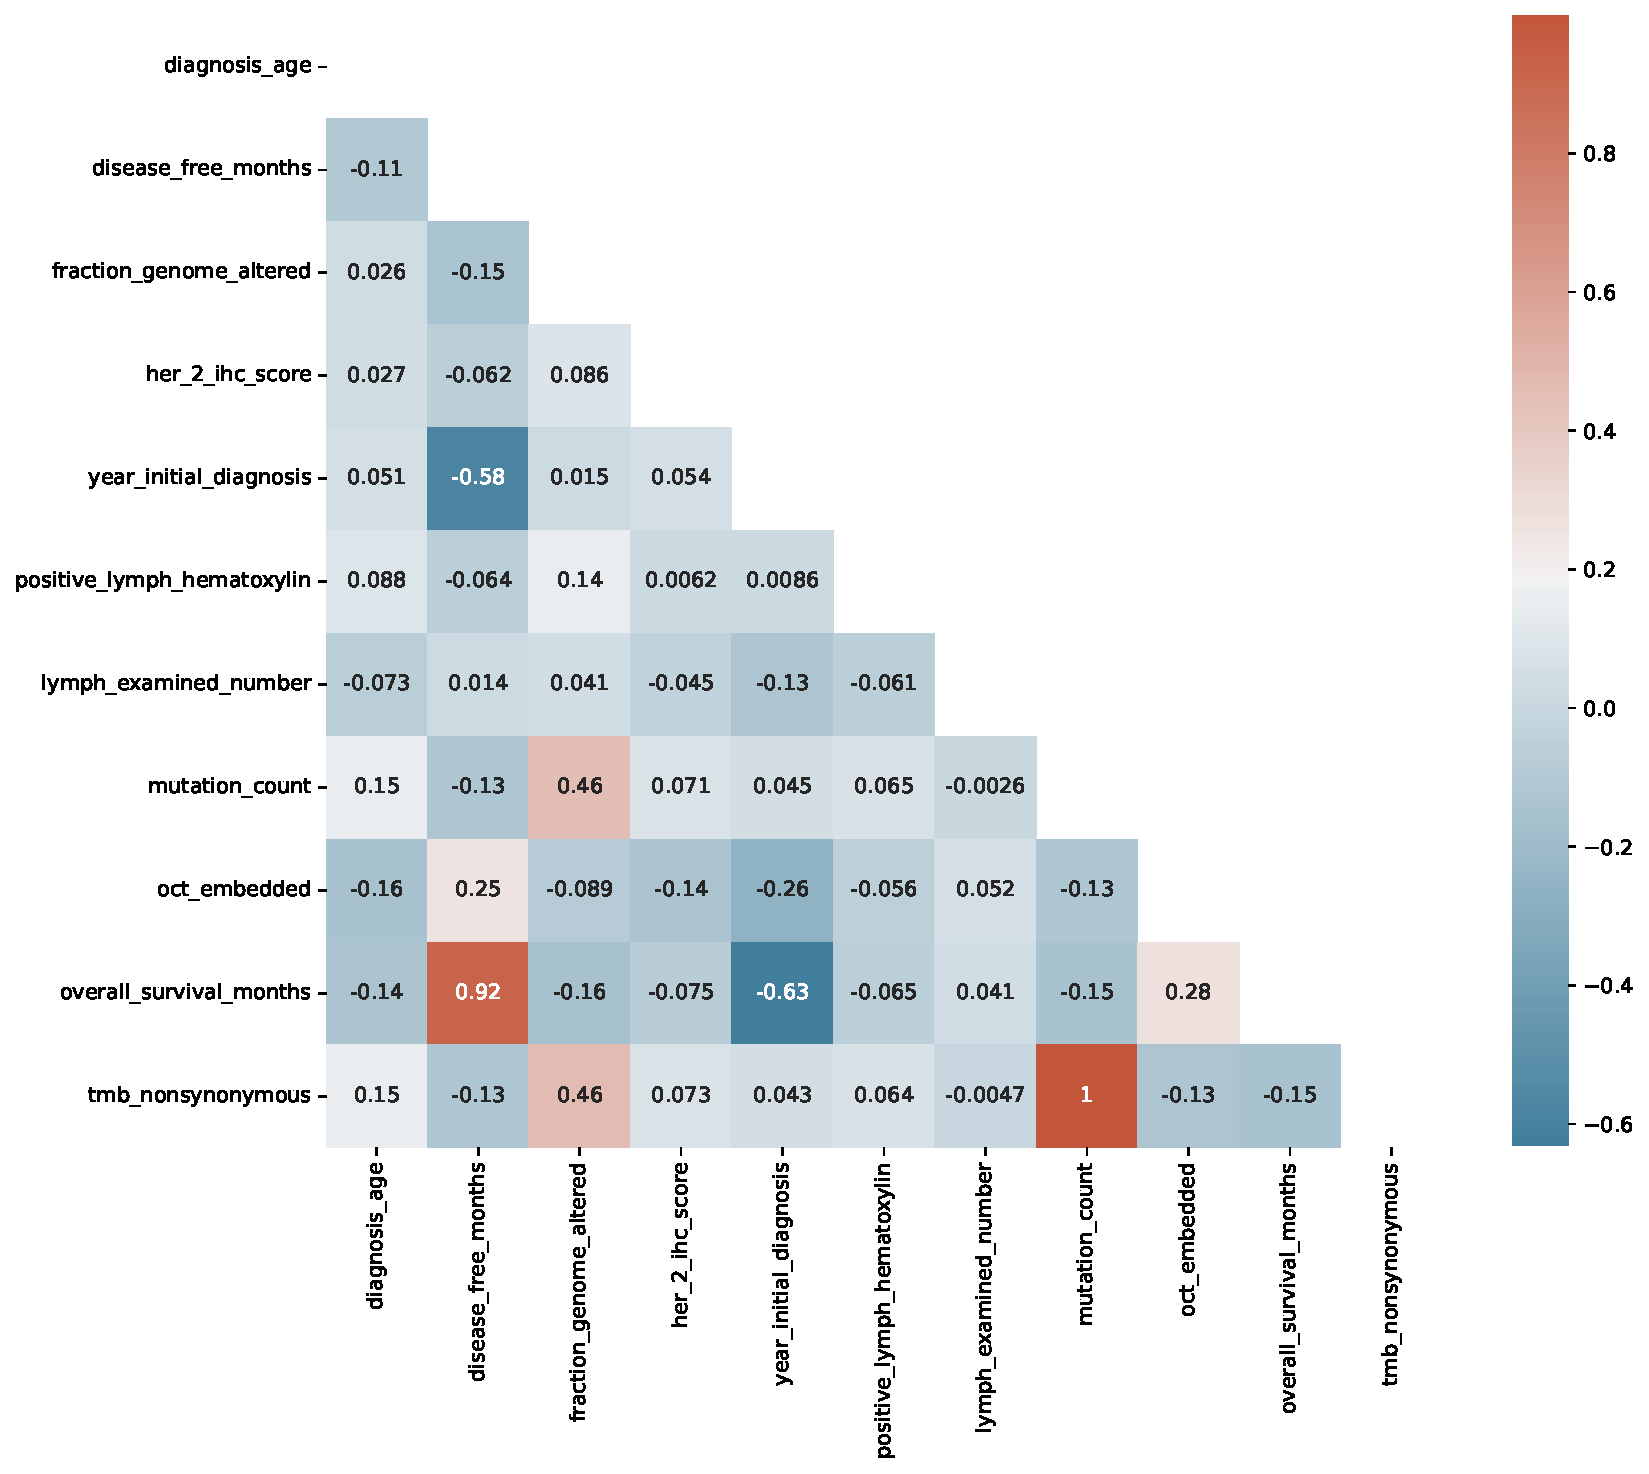
\includegraphics[width=1
	\linewidth]{NOTEBOOK/IMAGENES_CORRELACION/correlacion_spearman}
	\caption{Coeficiente de correlación de Spearman para el conjunto de datos “Breast Invasive Carcinoma (TCGA, Cell 2015)”}.
	\label{heatmap}
\end{figure}

En la figura \ref{analisis_correlacion} se puede observar el análisis realizado con base al coeficiente de correlación de Spearman. 

\begin{table*}[htb!]
	\footnotesize
	\begin{threeparttable}
		\begin{tabular}{p{0.5cm} p{7cm} p{6.5cm}} \toprule
			\begin{center}$N$\end{center}   	 
			&\begin{center}Análisis de correlación\end{center}             
			&\begin{center}Regresión lineal\end{center}\\ \hline
			1
			& Existe una correlación positiva del $100\%$ entre el \textit{recuento de mutaciones} y la \textit{carga mutacional tumoral (TMB)} del paciente. Por lo tanto, se infiere que entre mayor sea la cantidad de mutaciones presentadas en el ADN mayor será el rechazo del paciente ha determinado medicamento para ayudar a combatir el cáncer de mama.
			
			& \begin{center}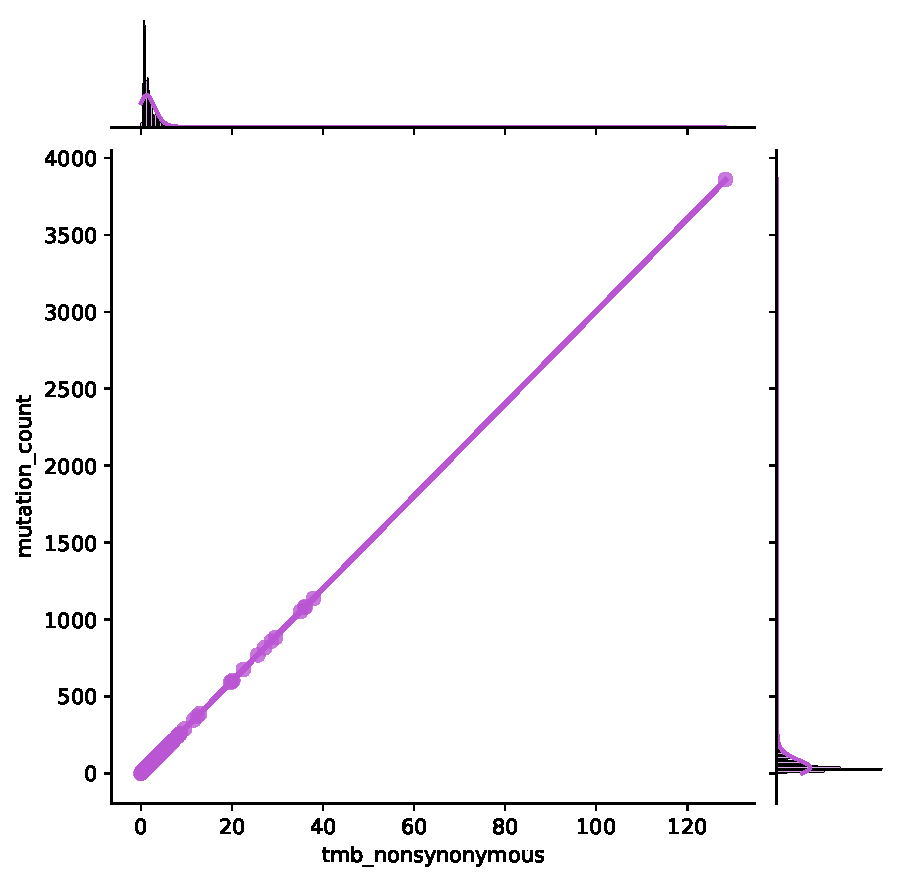
\includegraphics[width=1\linewidth]{NOTEBOOK/IMAGENES_CORRELACION/reg_tmb_nonsynonymous_mutation_count}\end{center}
			\\ \hline
			%------------------------------------------------------	
			2
			& Existe una correlación positiva del $92\%$ entre la \textit{supervivencia general} y el \textit{estado libre de enfermedad} del paciente. Por lo tanto, se infiere que para que el paciente tenga una mayor supervivencia a lo largo de los años no debe existir presencia del cáncer de mama. Por lo que es necesario que las biopsias garanticen la menor propagación de esta enfermedad desde el seno a otras partes del cuerpo.
			
			& \begin{center}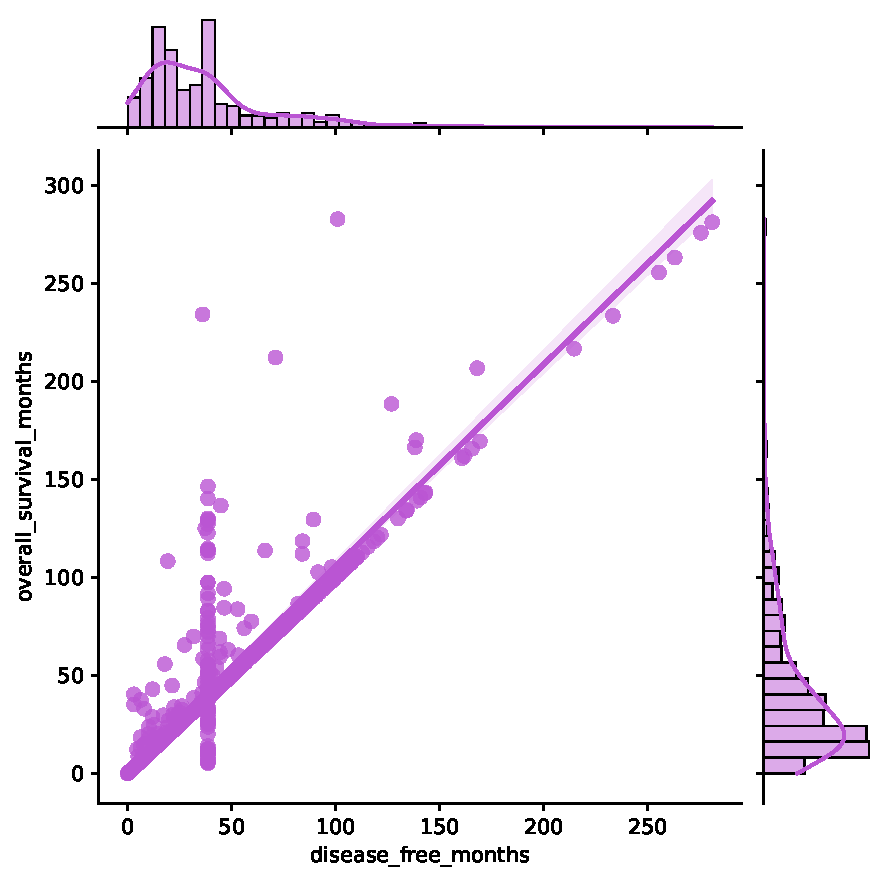
\includegraphics[width=1\linewidth]{NOTEBOOK/IMAGENES_CORRELACION/reg_disease_free_months_overall_survival_months}\end{center}
			\\ \hline
		\end{tabular}
		\caption{Análisis generando a partir de la correlación de Spearman.}
		\label{analisis_correlacion}
	\end{threeparttable}
\end{table*}
